\documentclass[a4paper, 11pt]{article}

\usepackage[utf8]{inputenc}
\usepackage[czech]{babel}
\usepackage[left=2cm, text={17cm, 24cm}, top=3cm]{geometry}
\usepackage[IL2]{fontenc}
\usepackage{palatino}
\usepackage{xcolor}
\usepackage{graphicx}\graphicspath{ {./img/} }

\definecolor{darkred}{rgb}{0.8,0,0}
\definecolor{blendedblue}{rgb}{0.2,0.2,0.7}
\definecolor{amber}{rgb}{1.0, 0.75, 0.0}
\definecolor{blue-violet}{rgb}{0.54, 0.17, 0.89}
\definecolor{coquelicot}{rgb}{1.0, 0.22, 0.0}
\colorlet{mixgreen}{green!50!black}


\begin{document}

\begin{titlepage}
	
	\begin{center}
	
	\begin{huge}
		
		\textsc{Vysoké učení technické v Brně}
		
		Fakulta informačních technologií
		
	\end{huge}
	
	\vspace{\stretch{0.382}}
	
	\begin{LARGE}
		
		Databázové systémy (IDS)
		
		Dokumentace popisující finální schéma databáze
		
		\bigskip
		
		\textbf{Zadání č. 52}
		
		\textbf{Portál hráčů Dračího doupěte}
		
	\end{LARGE}

	\end{center}
	
	\vspace{\stretch{0.618}}
	
	\begin{large}
		
%		\noindent Jakub Frýz (xfryzj01) \\ Jakub Hud (xhudja00) \hfill v Brně \today

		\noindent Jakub Frýz (\texttt{xfryzj01}) \hfill v Brně \\ Jakub Hud (\texttt{xhudja00}) \hfill \today
		
	\end{large}
	
\end{titlepage}

\tableofcontents

\pagebreak

\section{Zadání}

\begin{large}
	Fanoušci dračího doupěte si založili portál pro sdružení hráčské komunity. Systém umožňuje plánovat a evidovat jednotlivé sezení, základní informace o hráčích, jejich postavách a dobrodružstvích. \textcolor{coquelicot}{\textbf{Hráče}} charakterizují základní běžné informace o jeho \textcolor{coquelicot}{osobě}, \textcolor{coquelicot}{postavy}, které vlastní, či \textcolor{coquelicot}{sezení} a \textcolor{coquelicot}{dobrodružství}, kterých se v minulosti účastnil. \textcolor{coquelicot}{\textbf{Hráči}} mohou vlastnit několik \textcolor{coquelicot}{postav}, ze které vystupuje v konkrétních \textcolor{coquelicot}{dobrodružstvích}, přičemž v každém dobrodružství může vystupovat jako několik postav zároveň. \textcolor{blue-violet}{\textbf{Postavy}} mají určitou \textcolor{blue-violet}{úroveň}, různé \textcolor{blue-violet}{rasy} (ork, elf, půlelf, poloork, půlčík,…), \textcolor{blue-violet}{povolání} (válečník, mág, alchymista,…) a \textcolor{amber}{\textbf{vybavení}}, které buď zakoupila ve městě v obchodech, nebo obdržela během konkrétního dobrodružství o různé \textcolor{amber}{kvantitě} a různých \textcolor{amber}{typů} (zbraň, provize, šípy, apod.). Evidujte rovněž \textcolor{blue-violet}{smrti} jednotlivých postav, i \textcolor{blue-violet}{lokaci}, kde postava skonala (uvažujeme, že nelze postavy nijak oživit). \textcolor{mixgreen}{\textbf{Dobrodružství}} se konají v různých \textcolor{mixgreen}{lokalitách}, mají různé \textcolor{mixgreen}{obtížnosti}, jednoho i více \textcolor{mixgreen}{autorů} a herní \textcolor{mixgreen}{postavy}, které se jich účastní. Některé \textcolor{mixgreen}{\textbf{dobrodružství}} mohou být součástí \textcolor{blendedblue}{\textbf{tažení}}, které se odehrávají na celých \textcolor{blendedblue}{kontinentech} a sestávat z desítek menších \textcolor{blendedblue}{dobrodružství}. Každé \textcolor{blendedblue}{\textbf{tažení}} a \textcolor{mixgreen}{\textbf{dobrodružství}} má určitý \textcolor{blendedblue}{c}\textcolor{mixgreen}{íl}, jako například dobytí bašty, zabití monstra, nebo jen prozkoumání oblasti. Řada, z těchto dobrodružství je však příliš rozsáhlá, a tak jsou členěna do několika \textcolor{darkred}{\textbf{sezení}}, které se konají buď v dedikovaných hernách, nebo u hráčů doma. Systém pochopitelně poskytuje informaci o \textcolor{darkred}{počtu zúčastněných} hráčů. Jeden z hráčů je pak \textcolor{darkred}{Pánem Jeskyně} a vede dobrodružství, přičemž systém umožňuje PJovi zaslat pozvánky ostatním hráčům. Hráči si navíc mohou vytisknout statistiku o svých úspěších, počet zabití, počet obdrženého zlata apod.
\end{large}

\pagebreak

\section{Finální schéma databáze}

\subsection{Schéma}

\smallskip

\begin{figure}[h]
	\centering
	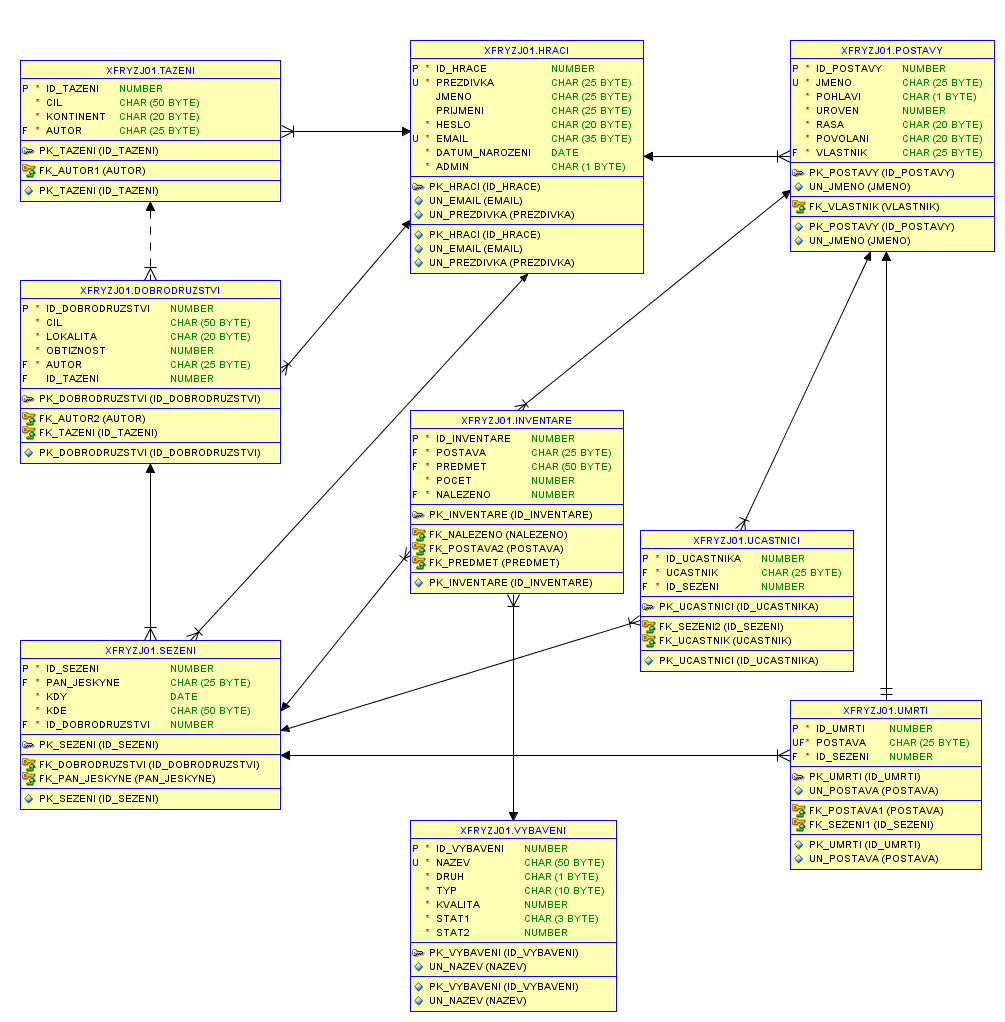
\includegraphics[width=0.95\textwidth]{erd}
\end{figure}


\subsection{Generalizace/specifikace}

Generalizaci/specifikaci jsme v naší databázi využili v tabulce \texttt{VYBAVENI} a to tak, že namísto spousty tabulek pro jednotlivé předměty (lektvary, zbraně, zbroje, \dots), které mají podobné atributy, máme pouze jednu entitu. Proto jsme i do tabulky \texttt{VYBAVENI} přidali atribut \texttt{TYP}, což je příznak, který určuje typ předmětu.

\pagebreak

\section{Implementace}

\subsection*{V \uv{kosce}}

Skript nejprve vytvoří sekvence a tabulky. Při tvorbě tabulek se určí, které atributy jsou primární klíče (\texttt{PRIMARY KEY}), unikátní (\texttt{UNIQUE}), nenulové (\texttt{NOT NULL}), které mají výchozí hodnotu (\texttt{DEFAULT}) a u kterých atributů je potřeba kontrola vstupních hodnot (\texttt{CHECK}). Poté, až jsou všechny tabulky vytvořeny, se nastaví cizí klíče (\texttt{FOREIGN KEY}).

V tuhle chvíli jsou už tabulky hotové, takže se vytvoří \uv{spouštěče}, procedury, apod. Pak se jenom udělí práva pro kolegu (\texttt{GRANT}).

Následuje vložení hodnot do tabulek (\texttt{INSERT}), výpisy z nich (\texttt{SELECT}) a spuštění procedur (\texttt{EXECUTE}).

\subsection{Spouštěče}

Skript obsahuje dva \uv{spouštěče}:

\begin{enumerate}
	\item \texttt{trigger\_participant}
		\begin{itemize}
			\item[--] Pokud hráč přihlašuje svoji postavu, která je mrtvá, vyhodí to chybu na výstup konzole. To stejné platí, pokud je postava k sezení už přihlášená.
		\end{itemize}
	\item \texttt{trigger\_participant}
		\begin{itemize}
			\item[--] Pomocí sekvence tvoří nový index pro tabulku \texttt{VYBAVENI}, pokud nebyl zadán.
		\end{itemize}
\end{enumerate}

\subsection{Procedury}

Skript obsahuje tyto procedury:

\begin{enumerate}
	\item \texttt{player\_stats(player IN VARCHAR2)}
		\begin{itemize}
			\item[--] Vypíše statistiky o zadaném hráči a jeho postavách. Pokud hráč neexistuje, procedura vyhodí chybu.  
			\item[--] Použítí kurzoru, datového typu odkazující se na řádek, ošetření výjimek
		\end{itemize}
	\item \texttt{upcoming\_sessions}
		\begin{itemize}
			\item[--] Vypíše všechna nadcházející sezení seřazená podle data konání.
			\item[--] Použítí kurzoru, datového typu odkazující se na řádek a typ sloupce.
		\end{itemize}
\end{enumerate}

\pagebreak

\subsection{Plán \& index}

\texttt{EXPLAIN PLAIN} jsme demonstrovali na jednoduchém příkazu \texttt{SELECT}. \texttt{EXPLAIN PLAN} neprovede samotný příkaz, ale ukáže \uv{plán}, jak tento příkaz databáze spouští s společně dalšími informacemi jako je např. zátěž na procesor. Tento \uv{plán} jsme si nechali vypsat dvakrát. Poprvé bez indexu a potom s indexem. Výsledkem jsou výpisy v tabulkách níže.

\begin{table}[h]
	\catcode`\-=12
	\centering
	\scriptsize
	\begin{tabular}{clccccc}
		\textbf{Id} & \multicolumn{1}{c}{\textbf{Operation}} & \textbf{Name} & \textbf{Rows} & \textbf{Bytes} & \textbf{Cost (\%CPU)} & \textbf{Time} \\ \hline
		0           & SELECT STATEMENT                       &               & 5             & 60             & 5 (40)                & 00:00:01      \\
		1           & SORT ORDER BY                          &               & 5             & 60             & 5 (40)                & 00:00:01      \\
		2           & HASH GROUP BY                          &               & 5             & 60             & 5 (40)                & 00:00:01      \\
		3           & TABLE ACCESS FULL                      & POSTAVY       & 6             & 72             & 3 (00)                & 00:00:01     
	\end{tabular}
	\normalsize
	\caption{\texttt{EXPLAIN PLAN} bez indexu}
\end{table}

\begin{table}[h]
	\catcode`\-=12
	\centering
	\scriptsize
	\begin{tabular}{clccccc}
		\textbf{Id} & \multicolumn{1}{c}{\textbf{Operation}} & \textbf{Name} & \textbf{Rows} & \textbf{Bytes} & \textbf{Cost (\%CPU)} & \textbf{Time} \\ \hline
		0           & SELECT STATEMENT                       &               & 5             & 60             & 4 (50)                & 00:00:01      \\
		1           & SORT ORDER BY                          &               & 5             & 60             & 4 (50)                & 00:00:01      \\
		2           & HASH GROUP BY                          &               & 5             & 60             & 4 (50)                & 00:00:01      \\
		3           & TABLE ACCESS BY INDEX ROWID BATCHED    & POSTAVY       & 6             & 72             & 2 (00)                & 00:00:01      \\
		4           & INDEX FULL SCAN                        & INDEX\_UROVEN & 6             &                & 1 (00)                & 00:00:01     
	\end{tabular}
	\normalsize
	\caption{\texttt{EXPLAIN PLAN} s indexem}
\end{table}

Z tabulek lze vyčíst, že sice provedení příkazu s indexem stálo méně zdrojů, ale zvýšila se zátěž na procesor.

\subsection{Materializovaný pohled}

Než se vytvoří materializovaný pohled jsme si prvně vytvořili materializovaný log, kde se uchovávají změny hlavní tabulky. Díky tomu můžeme použít \texttt{FAST REFRESH ON COMMIT}.

Součástí tvorby pohledu je i ukázka, že funguje. Po vytvoření si z něho necháme vypsat vše, co obsahuje, následně jsem přidali data do tabulky, ze které je pohled vytvořen, potvrdili změny pomocí \texttt{COMMIT} a zase jsme si nechali data vypsat.

Pohled jsme nastavili takto:

\begin{itemize}
	\item \texttt{CACHE}
	\begin{itemize}
		\item[--] bloky, které tato tabulka zabírá jsou uloženy na začátek vyrovnávací paměti, což urychluje jejich načtení
	\end{itemize}
	\item \texttt{BUILD IMMEDIATE}
	\begin{itemize}
		\item[--] hned, jak se pohled vytvoří, se naplní daty (není třeba \texttt{REFRESH})
	\end{itemize}
	\item \texttt{REFRESH FAST ON COMMIT}
	\begin{itemize}
		\item[--] pohled je aktualizován pomocí logů (není třeba celý pohled smazat a vytvořit znova), provede se při provedení \texttt{COMMIT}
	\end{itemize}
	\item \texttt{ENABLE QUERY REWRITE}
	\begin{itemize}
		\item[--] bude používán optimalizátorem
	\end{itemize}
\end{itemize}

\section{Závěr}

Skript byl tvořen a testován pomocí aplikace SQL Developer na školním serveru gort. K úspěšnému vypracování jsme použili dodané prezentace z předmětu IDS, oficiální dokumentaci na stránkách Oracle a jiné neoficiální stránky, především fóra (např. StackOverflow).

Databázi jsme se snažili zachovat co nejjednodušší, reálné provedení by bylo mnohem obsáhlejší.

\end{document}
